\section{Additional results}
\label{sec:S_results}

\subsection{Protocol P1 and oil saturation}
Table~\ref{tab:S_P1} repeats the fixed-rank P2 table in Section~\ref{sec:S_legacy} for protocol P1, and Table~\ref{tab:S_So} gives the oil-saturation errors in P2. The complete fold-level results for all budgets are in \texttt{outputs/e2\_summary.csv}, and the Wilcoxon tests in \texttt{outputs/stats\_wilcoxon.csv}.

\begin{table}[tbp]
\centering
\scriptsize
\setlength{\tabcolsep}{2.5pt}
\caption{As Table~\ref{tab:main}, for protocol P1 (within-scenario temporal hold-out; prior = persistence).}
\label{tab:S_P1}
\begin{adjustbox}{max width=\linewidth}
\begin{tabular}{@{}lcccccc@{}}
\toprule
 & \multicolumn{3}{c}{Grid-wide channels} & \multicolumn{2}{c}{Wells ($p$, $S_o$)} & Wells ($p$) \\
\cmidrule(lr){2-4}\cmidrule(lr){5-6}\cmidrule(l){7-7}
Method & $N=10$ & $N=30$ & $N=100$ & $N=10$ & $N=30$ & $N=30$ \\
\midrule
No measurements (prior) & 0.19\,$\pm$\,0.03 & 0.19\,$\pm$\,0.03 & 0.19\,$\pm$\,0.03 & 0.19\,$\pm$\,0.03 & 0.19\,$\pm$\,0.03 & 0.19\,$\pm$\,0.03 \\
Prior + IDW (POD-E sites) & 0.07\,$\pm$\,0.02 & 0.07\,$\pm$\,0.02 & 0.07\,$\pm$\,0.01 & 0.07\,$\pm$\,0.02 & 0.04\,$\pm$\,0.01 & 0.04\,$\pm$\,0.01 \\
POD, LS & 0.02\,$\pm$\,0.01 & 0.02\,$\pm$\,0.01 & 0.02\,$\pm$\,0.01 & 0.03\,$\pm$\,0.01 & 0.03\,$\pm$\,0.01 & 0.02\,$\pm$\,0.01 \\
POD, $\ell_1$ & 3.64\,$\pm$\,0.50 & 1.38\,$\pm$\,0.17 & 0.60\,$\pm$\,0.08 & 1.67\,$\pm$\,0.17 & 0.75\,$\pm$\,0.11 & 2.89\,$\pm$\,1.05 \\
POD-E, LS & 0.02\,$\pm$\,0.01 & 0.02\,$\pm$\,0.01 & 0.02\,$\pm$\,0.01 & 0.03\,$\pm$\,0.01 & 0.03\,$\pm$\,0.01 & 0.02\,$\pm$\,0.01 \\
POD-E, $\ell_1$ & 0.12\,$\pm$\,0.04 & 0.08\,$\pm$\,0.03 & 0.05\,$\pm$\,0.01 & 0.12\,$\pm$\,0.03 & 0.08\,$\pm$\,0.03 & 0.11\,$\pm$\,0.03 \\
TBMD $(48,48,2)$, LS & 0.47\,$\pm$\,0.14 & 0.36\,$\pm$\,0.07 & 0.31\,$\pm$\,0.04 & 0.39\,$\pm$\,0.08 & 0.34\,$\pm$\,0.03 & 0.32\,$\pm$\,0.03 \\
TBMD $(48,48,2)$, $\ell_1$ & 0.50\,$\pm$\,0.14 & 0.37\,$\pm$\,0.06 & 0.31\,$\pm$\,0.04 & 0.42\,$\pm$\,0.07 & 0.32\,$\pm$\,0.04 & 0.31\,$\pm$\,0.03 \\
Random sites, POD-E, LS & 0.17\,$\pm$\,0.07 & 0.04\,$\pm$\,0.02 & 0.02\,$\pm$\,0.00 & 0.05\,$\pm$\,0.01 & 0.03\,$\pm$\,0.01 & 0.02\,$\pm$\,0.01 \\
Configured wells, POD-E, LS & -- & -- & -- & 0.05\,$\pm$\,0.03 & 0.03\,$\pm$\,0.01 & 0.02\,$\pm$\,0.01 \\
Configured wells, TBMD, $\ell_1$ & -- & -- & -- & 0.31\,$\pm$\,0.03 & 0.32\,$\pm$\,0.04 & 0.31\,$\pm$\,0.03 \\
\bottomrule
\end{tabular}
\end{adjustbox}
\end{table}

\begin{table}[tbp]
\centering
\scriptsize
\setlength{\tabcolsep}{2.5pt}
\caption{Oil-saturation RMSE ($\times10^{-3}$) in protocol P2; layout as Table~2 of the main text. For pressure-only wells, $S_o$ is inferred through the joint basis.}
\label{tab:S_So}
\begin{tabular}{@{}lcccccc@{}}
\toprule
 & \multicolumn{3}{c}{Grid-wide channels} & \multicolumn{2}{c}{Wells ($p$, $S_o$)} & Wells ($p$) \\
\cmidrule(lr){2-4}\cmidrule(lr){5-6}\cmidrule(l){7-7}
Method & $N=10$ & $N=30$ & $N=100$ & $N=10$ & $N=30$ & $N=30$ \\
\midrule
No measurements (prior) & 839\,$\pm$\,213 & 839\,$\pm$\,213 & 839\,$\pm$\,213 & 839\,$\pm$\,213 & 839\,$\pm$\,213 & 839\,$\pm$\,213 \\
Prior + IDW (POD-E sites) & 2241\,$\pm$\,1500 & 2336\,$\pm$\,901 & 2041\,$\pm$\,702 & 1643\,$\pm$\,528 & 780\,$\pm$\,197 & 839\,$\pm$\,213 \\
POD, LS & 260237\,$\pm$\,3452 & 833\,$\pm$\,187 & 720\,$\pm$\,123 & 861\,$\pm$\,318 & 745\,$\pm$\,187 & 44023\,$\pm$\,25078 \\
POD, $\ell_1$ & 262436\,$\pm$\,5936 & 18164\,$\pm$\,3401 & 5102\,$\pm$\,1784 & 22641\,$\pm$\,2213 & 6358\,$\pm$\,1465 & 63565\,$\pm$\,8719 \\
POD-E, LS & 1158\,$\pm$\,355 & 804\,$\pm$\,179 & 719\,$\pm$\,122 & 822\,$\pm$\,185 & 745\,$\pm$\,187 & 44023\,$\pm$\,25078 \\
POD-E, $\ell_1$ & 2089\,$\pm$\,449 & 1318\,$\pm$\,178 & 797\,$\pm$\,138 & 1076\,$\pm$\,202 & 869\,$\pm$\,123 & 13268\,$\pm$\,3951 \\
TBMD $(48,48,2)$, LS & 6570\,$\pm$\,298 & 4733\,$\pm$\,294 & 4561\,$\pm$\,83 & 4508\,$\pm$\,183 & 4242\,$\pm$\,32 & 96362\,$\pm$\,58820 \\
TBMD $(48,48,2)$, $\ell_1$ & 6707\,$\pm$\,596 & 4677\,$\pm$\,266 & 4575\,$\pm$\,81 & 4353\,$\pm$\,63 & 4251\,$\pm$\,24 & 15550\,$\pm$\,6471 \\
Random sites, POD-E, LS & 2251\,$\pm$\,584 & 2579\,$\pm$\,699 & 847\,$\pm$\,132 & 1699\,$\pm$\,445 & 745\,$\pm$\,187 & 44023\,$\pm$\,25078 \\
Configured wells, POD-E, LS & -- & -- & -- & 2787\,$\pm$\,1517 & 745\,$\pm$\,187 & 44023\,$\pm$\,25078 \\
Configured wells, TBMD, $\ell_1$ & -- & -- & -- & 4686\,$\pm$\,98 & 4251\,$\pm$\,24 & 15550\,$\pm$\,6471 \\
\bottomrule
\end{tabular}
\end{table}


\subsection{Joint versus independent property modelling (E8)}
The channel ablations in E2 change observations while retaining a joint basis; they do not isolate joint model fitting. E8 therefore fits two independent third-order space--space--time TBMD models, using exactly the P1/P2 training splits, property-wise scaling, spatial ranks $(48,48)$ and estimators used for joint fourth-order TBMD. Each comparison uses identical pressure and saturation measurements at the first 10 or all 30 configured wells (20 or 60 scalar channels). No placement is re-optimised. For the training-selected joint depth $r$, one independent control assigns $\lfloor r/2\rfloor$ pressure coefficients and $r-\lfloor r/2\rfloor$ saturation coefficients (equal total capacity); another assigns $r$ to each property (equal per-property capacity, twice the total). Independent bases form a block-diagonal dictionary; the same LS or $\ell_1$ objective then separates by property. E8 changes both the shared spatial representation and the use of shared coefficients, so its performance difference cannot be attributed to either mechanism alone. Both capacity controls are reported without test-set tuning; no additional held-out-driven ablation was introduced to search for a configuration favourable to the joint model.

Table~\ref{tab:S_coupling} reports the all-well P2 comparison. Both independent controls have lower mean errors for both variables than joint TBMD with either estimator. The equal-total control also avoids the doubled coefficient count of the per-property control. These results establish no benefit of the original enforced joint structure for this setting, not a universal disadvantage of property coupling. E9 (Supplementary Section~\ref{sec:S_e9}) preserves this negative comparator and then tests anomaly/structural metrics, nested tuning and partially shared architectures; it does not overwrite E8. The complete 240 E8 fold/design records, including P1 and the 10-well comparison, are in \texttt{e8\_property\_coupling.csv}; the table is generated by \texttt{e8\_property\_coupling.py}, not transcribed manually.

% Generated by e8_property_coupling.py; do not edit.
\begin{table}[htbp]\centering\small
\caption{Matched-measurement property-coupling ablation (E8), P2, all 30 wells (60 channels). Mean $\pm$ sample standard deviation over ten held-out scenarios; RMSE is averaged over snapshots within each fold. All models use the same measurements and spatial ranks $(48,48)$. The two independent controls use equal total or equal per-property coefficient counts.}
\label{tab:S_coupling}
\begin{tabular}{lrrr}\toprule
Model / estimator & Coefficients & Pressure ($u_p$) & $S_o$ ($10^{-3}$) \\\midrule
Independent, total / $\ell_1$ & 16 & $0.262 \pm 0.078$ & $0.984 \pm 0.216$ \\
Independent, total / LS & 16 & $0.275 \pm 0.079$ & $0.741 \pm 0.162$ \\
Independent, per property / $\ell_1$ & 32 & $0.261 \pm 0.079$ & $0.985 \pm 0.216$ \\
Independent, per property / LS & 32 & $0.360 \pm 0.091$ & $1.870 \pm 0.909$ \\
Joint 4D / $\ell_1$ & 16 & $0.432 \pm 0.060$ & $4.251 \pm 0.024$ \\
Joint 4D / LS & 16 & $0.432 \pm 0.050$ & $4.242 \pm 0.032$ \\
\bottomrule\end{tabular}\end{table}


\subsection{Spatial structure of the scenario deviation and of truncation errors (E7)}
For every P2 fold, the deviation of the held-out scenario from the ensemble-mean prior has a mean absolute field-wide shift of \DevShiftMin--\DevShiftMax{} $u_p$ and a spatial standard deviation of \DevSdMin--\DevSdMax{} $u_p$ (averaged over snapshots). The absolute deviation from the field-wide shift is negatively correlated with the distance to the nearest well (Pearson correlation $\DevCorrMin$ to $\DevCorrMax$). With full observation, the per-cell RMSE of TBMD $(48,48,2)$ averages \OracleTbmdNear{} $u_p$ within two cells of a well and \OracleTbmdFar{} $u_p$ more than ten cells away; the corresponding POD values are \OraclePodNear{} and \OraclePodFar{} $u_p$ (\texttt{outputs/e7\_spatial\_structure.csv}).

\subsection{Sensitivity to the $\ell_1$ weight (E4)}
Figure~\ref{fig:S_l1} shows the pressure error of the $\ell_1$ estimator over the tested weights $\varepsilon$ (Section~\ref{sec:S_legacy}).
\begin{figure}[htbp]
\centering
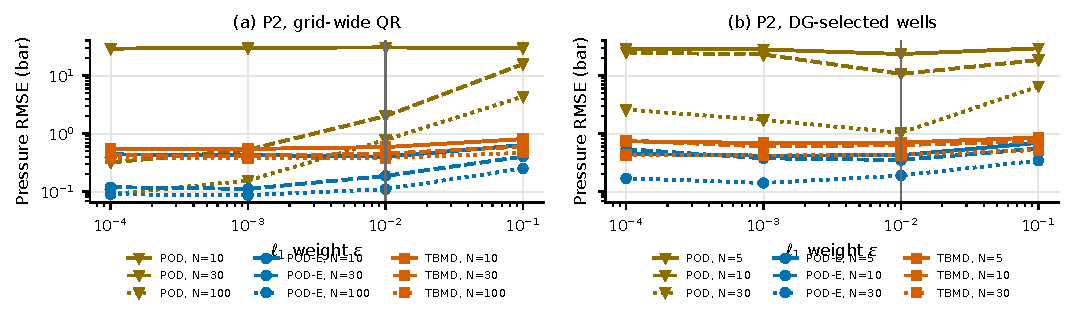
\includegraphics[width=\textwidth]{../../../../studies/brugge_sparse_sensing/figures/figS1_l1_sensitivity.pdf}
\caption{P2 pressure RMSE of the $\ell_1$ estimator against $\varepsilon$ for (a) QR-selected grid channels ($N=10,30,100$) and (b) DG-selected wells ($N=5,10,30$), for POD, POD-E and TBMD $(48,48,2)$ bases. Line style distinguishes budgets; the vertical line marks $\varepsilon=10^{-2}$.}
\label{fig:S_l1}
\end{figure}

\subsection{Example reconstruction}
Figure~\ref{fig:S_maps} shows error maps for one held-out scenario and snapshot.
\begin{figure}[htbp]
\centering
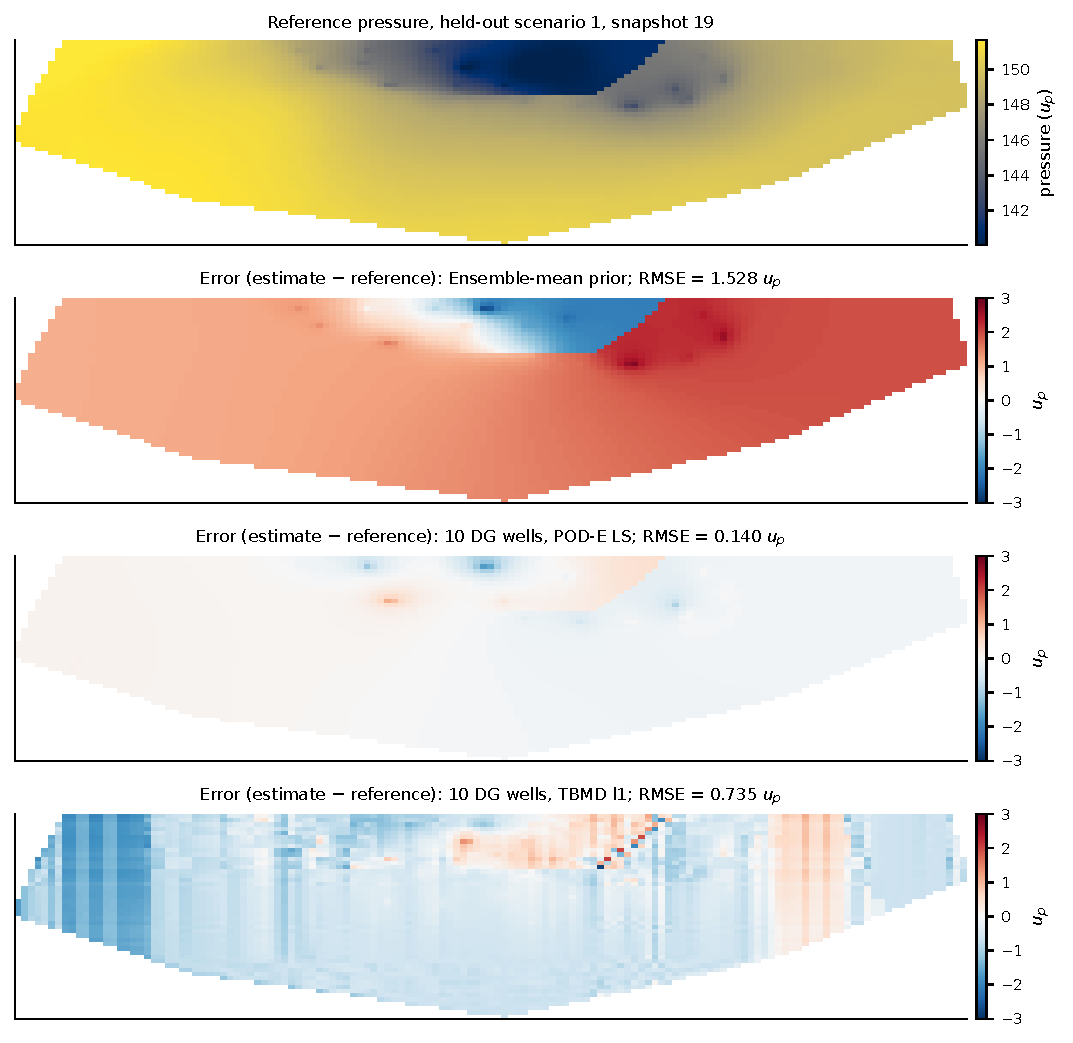
\includegraphics[width=\textwidth]{../../../../studies/brugge_sparse_sensing/figures/figS2_example_maps.pdf}
\caption{Reference pressure of held-out scenario 1 (P2) at the snapshot with the largest cross-scenario spread, and signed errors (estimate minus reference, in $u_p$) of the ensemble-mean prior and of reconstructions from ten DG-selected wells (pressure and $S_o$) with POD-E least squares and with TBMD $(48,48,2)$ $\ell_1$. The panel titles give the RMSE of each map.}
\label{fig:S_maps}
\end{figure}

\subsection{Stability of selections (E5)}
Table~\ref{tab:S_stab} summarises how consistently each basis selects channels and ranks wells across the ten leave-one-out folds.
\begin{table}[htbp]
\centering
\small
\caption{Stability and location of QR selections across the ten P2 leave-one-out bases (\texttt{outputs/e5\_stability.csv}) and Kendall rank correlation of DG well orders.}
\label{tab:S_stab}
\begin{adjustbox}{max width=\linewidth}
\begin{tabular}{@{}lcccccc@{}}
\toprule
Basis & \multicolumn{2}{c}{Mean Jaccard} & \multicolumn{2}{c}{Pressure share (\%)} & Distance to well, $N=50$ & Kendall $\tau$ (wells) \\
 & $N=r$ & $N=50$ & $N=r$ & $N=50$ & (cells) & mean (min) \\
\midrule
POD & \StabJacPodR & \StabJacPodFifty & \StabSharePPodR & \StabSharePPodFifty & \StabDistPodFifty & \StabTauPod{} (\StabTauMinPod) \\
POD-E & \StabJacPodeR & \StabJacPodeFifty & \StabSharePPodeR & \StabSharePPodeFifty & \StabDistPodeFifty & \StabTauPode{} (\StabTauMinPode) \\
TBMD & \StabJacTbmdR & \StabJacTbmdFifty & \StabSharePTbmdR & \StabSharePTbmdFifty & \StabDistTbmdFifty & \StabTauTbmd{} (\StabTauMinTbmd) \\
\bottomrule
\end{tabular}
\end{adjustbox}
\end{table}
The mean distance from an active cell to the nearest well is \StabDistActive{} cells.
